%   % !TEX root = ../../VIII,3_Rahmen-TeX_8-1.tex
%
%
%   Band VIII, 3 N.~??A34.2
%   Signatur/Tex-Datei: LH_35_14_02_161-162
%   RK-Nr. 58256 [Teil 1 ??]
%   Überschrift: De motu elaterii se restituentis
%   Modul: Mechanik / AEF (Elastizität)
%   Datierung: [Anfang August bis zweite Hälfte November 1689]
%   WZ: LEdWZ 803044 = RK-WZ 125 // 40l
%   SZ: \pleibvdash; \pleibdashv (insgesamt: zwei)
%   Bilddateien (PDF): LH_35_14_02_161-162_d1; LH_35_14_02_161-162_d2 (insgesamt: zwei)
%
%
\selectlanguage{ngerman}%
\frenchspacing%
%
\begin{ledgroupsized}[r]{120mm}%
\footnotesize%
\pstart%
\noindent\textbf{Überlieferung:}%
\pend%
\end{ledgroupsized}%
\begin{ledgroupsized}[r]{114mm}%
\footnotesize%
\pstart \parindent -6mm
\makebox[6mm][l]{\textit{L}}%
Aufzeichnung: LH~XXXV~14,~2 Bl.~161\textendash162.
Ein Bogen 8\textsuperscript{o};
Fragment eines Wasserzeichens auf Bl.~162:
italienisches Papier.
Drei Seiten;
Textfolge: Bl.~162~v\textsuperscript{o}, 161~r\textsuperscript{o} und 161~v\textsuperscript{o}.
Auf Bl.~161~v\textsuperscript{o}\! und 162~r\textsuperscript{o}\! ist N.~28\textsubscript{1} überliefert;
auf Bl.~162~r\textsuperscript{o} zudem ein mit dem Brief \textit{LSB} I,~5 N.~250\cite{01297} zusammenhängendes Textfragment (oben, S.~\refpassage{LH_35_14_02_162r_Brieffragment_hcyg-1}{LH_35_14_02_162r_Brieffragment_hcyg-2}).
\pend%
\end{ledgroupsized}%
%
% \vspace{5mm}%
% \begin{ledgroup}%
% \footnotesize%
% \pstart%
% \noindent\textbf{Datierungsgründe:}
% Das auf Bl.~162~r\textsuperscript{o} überlieferte, vom Text N.~??A35 überschriebene Fragment ist der Anfang eines ersten Entwurfes zum Brief, den Leibniz am 6. August 1689 aus Rom an C.~Gudenus, kurmainzischen Residenten in Wien, gesendet hat (\textit{LSB} I,~5 N.~250\cite{01297}; vgl. bes. S.~46.8\textendash10).
% Der Träger der Texte N.~??A34 und N.~??A35 weist auch das gleiche Wasserzeichen wie die Handschrift LBr~425 Bl.~57\textendash58 auf, die das vollständige Konzept des genannten Briefes überliefert.
% Entstanden sind N.~??A34 und N.~??A35 demnach wohl zwischen August 1689 und Leibnizens Abreise von Rom im November desselben, wahrscheinlich aber noch Anfang August. 
% \pend%
% \end{ledgroup}%
%
%
\selectlanguage{latin}%
\frenchspacing%
%
\vspace{8mm}%
%
%
\count\Bfootins=1100
\count\Afootins=1200
\count\Cfootins=1200
%
%
\pstart%
\noindent%
\normalsize%
%
\lbrack162~v\textsuperscript{o}\rbrack\ % Blatt 162v
\pend%
%
\pstart%
\noindent%
\centering%
De motu Elaterii se \edlabel{LH_35_14_02_161-162_e161r1}restituentis%
\protect\index{Sachverzeichnis}{elaterium}%
\protect\index{Sachverzeichnis}{elaterium se restituens}%
\protect\index{Sachverzeichnis}{motus elaterii}%
\protect\index{Sachverzeichnis}{motus restitutionis}%
\edtext{}{%
{\xxref{LH_35_14_02_161-162_e161r1}{LH_35_14_02_161-162_e161r2}}%
{\lemma{restituentis}\Bfootnote{%
\textit{(1)}~Spati
\textit{(2)}~Velocitates sunt ut spatia\protect\index{Sachverzeichnis}{velocitas restitutionis}
\textit{(a)}~. Ergo
\textit{(b)}~. Jam
\textit{(c)}~seu \textit{v} ut \textit{s}. Jam $d\overline{s}$
\textit{(aa)}~ut \textit{dv}
\textit{(bb)}~ut $d\overline{t}\,v.$ Ergo \textit{dt} ut $d\overline{s} : s.$
\textit{(aaa)}~Cumque
\textit{(bbb)}~In casu velo
\textit{(3)}~\textit{dv} sunt \lbrack...\rbrack\ ut $c^{ds} - s^{ds}.$ % ut spatia residua seu \textit{dv}
\textit{(a)}~Jam
\textit{(b)}~Ergo \textit{v} ut $cs-\displaystyle\frac{1}{2}ss.$
\textit{(aa)}~Ergo
\textit{(aaa)}~\textit{dt}
\textit{(bbb)}~\textit{t} ut
\textit{(bb)}~Ergo
\textit{(aaa)}~\textit{dt} ut
\textit{(bbb)}~\textit{dt} ut%
~\textit{L}}}}%
\pend%
%
%
%%  \newpage
%  \vspace{2.0em}%
%  \centerline{\hspace*{-50mm}\includegraphics[width=0.18\textwidth]{gesamttex/edit_VIII,3/images/LH_35_14_02_161-162_d1.pdf}}%
%  \vspace{0.0em}%
%  \centerline{\hspace*{-50mm}\lbrack\textit{Fig.~1}\rbrack}%
%  \label{LH_35_14_02_162v_Fig.1}%
%%  \vspace{1.5em}%
%%
%%
%%  \newpage
%  \vspace{-11.0em}%
%  \centerline{\hspace*{50mm}\includegraphics[width=0.21\textwidth]{gesamttex/edit_VIII,3/images/LH_35_14_02_161-162_d2.pdf}}%
%  \vspace{0.0em}%
%  \centerline{\hspace*{50mm}\lbrack\textit{Fig.~2}\rbrack}%
%  \label{LH_35_14_02_162v_Fig.2}%
%  \vspace{1.5em}%
%%  \newpage
%
%
\pstart%
\noindent%
\textit{dv} sunt ut spatia residua%
\protect\index{Sachverzeichnis}{spatium residuum}\protect\index{Sachverzeichnis}{spatium restitutionis}
seu \textit{dv} ut $c^{ds} - s^{ds}.$
Ergo \textit{v} ut $\displaystyle cs - \frac{1}{2}ss.$
Ergo\protect\rule[-2mm]{0mm}{10mm} \textit{dt} ut $\displaystyle ds : \overline{cs - \frac{1}{2}ss}.$\edlabel{LH_35_14_02_161-162_e161r2}
%
$d\overline{t}\; \overline{c - s} = dds$
seu $dds : \overline{c - s}= d\overline{t}\,ds$
seu $dt = d\overline{ds} \cdot d\overline{s} : \overline{c - s}.$
\protect\rule[-3mm]{0mm}{8mm}Aliter:\protect\index{Sachverzeichnis}{tempus restitutionis}
\textit{AT} sit tempus[,]
spatium residuum%
\protect\index{Sachverzeichnis}{spatium residuum}\protect\index{Sachverzeichnis}{spatium restitutionis}
%
\edtext{sit \textit{TR}.
Conatus impressus\protect\index{Sachverzeichnis}{conatus impressus}
novus\protect\index{Sachverzeichnis}{conatus novus}
percurrendi elementum spatii, \textit{ER},%
\protect\index{Sachverzeichnis}{elementum spatii}\protect\index{Sachverzeichnis}{spatium percurrendum}
erit \hspace{0.1mm}ut \hspace{0.1mm}\textit{TR}.
\hspace{0.1mm}Et \hspace{0.1mm}integra}{%
\lemma{sit \textit{TR}.}\Bfootnote{%
\textit{(1)}~Ponamus tempus in aequales partes esse divisum \textit{{\scriptsize{1}}T{\scriptsize{2}}T}
\textit{(2)}~Con
\textit{(3)}~Ponamus tempus
\textit{(4)}~Conatus impressus
\textbar~novus \textit{erg.}~%
\textbar\ percurrendi elementum spatii, \textit{ER},
\textit{(a)}~erit ut \textit{{\scriptsize{1}}T{\scriptsize{2}}T}
\textit{(aa)}~conatus int
\textit{(bb)}~seu si
\textit{(b)}~erit ut \textit{TR}. Et
\textbar~jam \textit{gestr.}~%
\textbar\ integra%
~\textit{L}}}
%
\hspace{0.1mm}\protect\rule[-3mm]{0mm}{8mm}velocitas\protect\index{Sachverzeichnis}{velocitas integra}\protect\index{Sachverzeichnis}{velocitas restitutionis}
\hspace{0.1mm}est \hspace{0.1mm}ut \hspace{0.1mm}$\displaystyle\!\!\int\!\!\overline{TR}\,dt.$
\hspace{0.1mm}Quae \hspace{0.1mm}est \hspace{0.1mm}ut \hspace{0.1mm}\textit{ER}.
\hspace{0.1mm}Ergo \hspace{0.1mm}fit
\edtext{\hspace{0.1mm}\textit{ER} \hspace{0.1mm}ut \hspace{0.1mm}$\displaystyle\!\!\int\!\!\!\!\!\int\!\!ER$}{%
\lemma{fit}\Bfootnote{%
\textit{(1)}~\textit{ER} ut
\textit{(2)}~\textit{ds}
\textit{(3)}~\textit{ER} ut% $\displaystyle\!\!\int\!\!\!\!\!\int\!\!ER$
~\textit{L}}}
\pend
\vspace{2.0em}
\pstart\hspace{15mm}
\begin{minipage}[t]{0.5\textwidth}
\includegraphics[width=0.37\textwidth]{gesamttex/edit_VIII,3/images/LH_35_14_02_161-162_d1.pdf}
\end{minipage}
\hspace{-5mm}\begin{minipage}[t]{0.5\textwidth}
\includegraphics[width=0.42\textwidth]{gesamttex/edit_VIII,3/images/LH_35_14_02_161-162_d2.pdf}
\end{minipage}
\\
\\
\hspace*{28mm} [\textit{Fig.~1}] \label{LH_35_14_02_162v_Fig.1}\hspace*{54mm} [\textit{Fig.~2}] \label{LH_35_14_02_162v_Fig.2}
\pend
\newpage
\pstart
\noindent
%
seu ut $\displaystyle\!\!\int\!\!TR.$
%
\edtext{Seu si sit spatium residuum $c - s,$%
\protect\index{Sachverzeichnis}{spatium residuum}\protect\index{Sachverzeichnis}{spatium restitutionis}
fiet}{%
\lemma{Seu}\Bfootnote{%
\textit{(1)}~fiet
\textit{(2)}~si sit \lbrack...\rbrack\ $c-s,$ fiet% spatium residuum
~\textit{L}}}\protect\rule[-3mm]{0mm}{8mm}
%
$ER = -\,ds,$ et fiet $-\,ds$ ut
%
\edtext{$\displaystyle\!\!\int\!\!\overline{\overline{c-s}}\,dt$ et $d\overline{ds}:\overline{c-s}$ ut $d\overline{t}.$}{%
\lemma{$\displaystyle\!\!\int\!\!\overline{\overline{c-s}}dt$}\Bfootnote{%
\textit{(1)}~seu $-\,dds$ ut $\overline{c-s}$ \textit{dt}. Ergo pro \textit{ds} ponendo
\textit{(a)}~\textit{dt}
\textit{(b)}~$\omega dt$
\textit{(aa)}~fiet
\textit{(bb)}~et \textit{dt}
\textit{(cc)}~et $\displaystyle\!\!\int\!\!\overline{\omega dt}=s$ fiet $-\,d\overline{\omega}=$
\textit{(aaa)}~$\overline{c-s}dt.$
\textit{(bbb)}~$\displaystyle c-\!\!\int\!\!\overline{\omega dt}dt$ et $-\,dd\omega =$
\textit{(2)}~et $d\overline{ds}:\overline{c-s}$ ut $d\overline{t}.$%
~\textit{L}}}
%
Quae aequatio\protect\index{Sachverzeichnis}{aequatio} a priore diversa est,
\edlabel{LH_35_14_02_162v_Hooke_dfhs-1}%
non igitur consentient
\edtext{Hookiana\protect\index{Namensregister}{\textso{Hooke} (Hookius, Hook), Robert 1635\textendash1703}}{%
\lemma{Hookiana}\Cfootnote{%
Wohl Anspielung auf R.~\textsc{Hooke}, \textit{Lectures de potentia restitutiva}, London 1678, S.~16\textendash22.\cite{01241}
Hierauf bezieht sich Leibniz kritisch auch in N.~25, S.~\refpassage{LH_35_10_08_019r_Hooke-1}{LH_35_10_08_019r_Hooke-2}.}}
%
cum meis.\edlabel{LH_35_14_02_162v_Hooke_dfhs-2}
Eadem si pro spatio%
\protect\index{Sachverzeichnis}{spatium residuum}\protect\index{Sachverzeichnis}{spatium restitutionis}
adhibeantur gradus dimensionis.\protect\index{Sachverzeichnis}{dimensio}\protect\index{Sachverzeichnis}{gradus dimensionis}
%
\lbrack161~r\textsuperscript{o}\rbrack\ % Blatt 161r
%
\pend%
%
%
\pstart%
Problema\protect\index{Sachverzeichnis}{problema trascendentium} hujusmodi
%
\edtext{Transcendentium,\protect\index{Sachverzeichnis}{trascendens}
quaeritur series\protect\index{Sachverzeichnis}{series} in qua \textit{ds}}{%
\lemma{Transcendentium,}\Bfootnote{%
\textit{(1)}~ut sint \textit{d}
\textit{(2)}~quaeritur series in qua \textit{ds}%
~\textit{L}}}
%
ut \textit{s}, vel \textit{ds} ut $1 : s^e\!.$ % \lbrack;\rbrack\
Solvi posse constat,
sed supersunt adhuc solvenda problemata
in quibus \textit{dds} ut $1 : s^e\!,$ vel aliter,
seu in quibus $d\overline{ds}\,s^e$ ut \textit{dt}.
Ponuntur autem \textit{dt}
%
\edtext{progressionis arithmeticae,\protect\index{Sachverzeichnis}{progressio arithmetica}}{%
\lemma{progressionis}\Bfootnote{%
\textit{(1)}~geometricae\protect\index{Sachverzeichnis}{progressio geometrica}
\textit{(2)}~arithmeticae,%
~\textit{L}}}
%
alioqui nec intelligeretur satis problema,\protect\index{Sachverzeichnis}{problema indeterminatum}
essetque indeterminatum.%
%%%%%%%%%%%%%%%%%%%%%%%%%
\pend%
\vspace{1mm}
\pstart%
\noindent%
%% \\
%\edtext{}{%
%{\xxref{LH_35_14_02_161r_kughauzdgf-1}{LH_35_14_02_161r_kughauzdgf-2}}%
%{\lemma{$ds\ =$}\Bfootnote{%
%\textit{(1)}~\textit{dt}, in
%\textit{(2)}~$11\; +$%
%~\textit{L}}}}%
\par\centering%
\begin{edtabularr}%
Sit $s\ =$ & $10\, t^0 + 11\, t^1\, +$ & $12\,t^2\, +$ & $13\,t^3$ etc. & \hfill \\
\hspace{-1.3mm}erit \hspace{2,0mm}\edlabel{LH_35_14_02_161r_kughauzdgf-1}$ds\ =$ & $11\; +$\edlabel{LH_35_14_02_161r_kughauzdgf-2} & $2 \cdot 12\,t\; +$ & $3 \cdot 13\,t^2$ etc. & \hfill \\
\hspace{-1.3mm}et \hspace{2,5mm}$dds\ =$ & $+$ & $1 \cdot 2\cdot 12\; +$ & $2 \cdot 3 \cdot 13\,t + 3 \cdot 4 \cdot 14\,t^2$ etc. & \hfill
%\edrowfill{1}{1}{\hspace{7mm}Sit} & $s\ =$ & $10\, t^0 + 11\, t^1\, +$ & $12\,t^2\, +$ & $13\,t^3$ etc. & \hfill \\
%\edrowfill{1}{1}{\hspace{1,1mm}erit} & \edlabel{LH_35_14_02_161r_kughauzdgf-1}$ds\ =$ & $11\; +$\edlabel{LH_35_14_02_161r_kughauzdgf-2} & $2 \cdot 12\,t\; +$ & $3 \cdot 13\,t^2$ etc. & \hfill \\
%\edrowfill{1}{1}{\hspace{1,1mm}et} & $dds\ =$ & $+$ & $1 \cdot 2\cdot 12\; +$ & $2 \cdot 3 \cdot 13\,t + 3 \cdot 4 %\cdot 14\,t^2$ etc. & \hfill
\ignorespacesafterend%
\end{edtabularr}%
\pend%
%
\pstart%
\noindent%
\setline{11}et $dd\overline{s}\cdot s - 1 = 0 = \hspace{8,05mm}-1$ \hfill%
\pend%
%
\pstart%
\noindent%
\par\centering%

\begin{edtabularl}
\hfill $1 \cdot 2 \cdot 12 \cdot 10$ & $+\;2 \cdot 3 \cdot 13 \cdot 10\,t$ & $+\;3 \cdot 4 \cdot 14 \cdot 10\,t^2 + 4 \cdot 5 \cdot 15 \cdot 10\,t^3$ \\%
\hfill & $\phantom{+\ }1 \cdot 2 \cdot 12 \cdot 11\,t$ & $\phantom{+\ }2 \cdot 3 \cdot 13 \cdot 11\,t^2 + 3 \cdot 4 \cdot 14 \cdot 11\,t^3$ \\%
\hfill & & $\phantom{+\ }1 \cdot 2 \cdot 12 \cdot 12\,t^2 + 2 \cdot 3 \cdot 13 \cdot 12\,t^3$ etc.%
\ignorespacesafterend%
\end{edtabularl}
\pend%

%
\pstart%
\noindent%
%%%%%%%%%%%%%%%%%%%%%%%%%%%%%%%%%%%%%%%%%%%%%%%%%%%
\par\centering%
\begin{edtabularl}%
ergo & \hspace{-3mm}$12=1:\overline{1\cdot 2\cdot 10}$ \hfill \\%
et & \hspace{-3mm}$13=-11:\overline{2\cdot 3}\cdot10^2$ \hfill \\%
et & \hspace{-3mm}$14=-2\cdot 3$ \hspace{2mm}
\lbrack\textit{Text bricht ab}.\rbrack\hspace{2mm}
%
\lbrack161~v\textsuperscript{o}\rbrack\ % Blatt 161v
%
\hfill%
\ignorespacesafterend%
\end{edtabularl}%
\pend%
%
\pstart%
$dds=c-s$ fiet
\pend%
% \vspace{0.2em}
%
\pstart%
\noindent%
\par\centering%
\begin{edarrayr}%
+ & 1 \cdot 2 \cdot 12 & +\ 2 \cdot 3 \cdot 13\,t & +\ 3 \cdot 4 \cdot 14\,t^2 & +\ 4 \cdot 5 \cdot 15\,t^3 \ \text{etc.} & \hspace{-3mm} \\
+ & c & -\ 11\,t & -\ 12\,t^2 & -\ 13\,t^3 \ \text{etc.} & \hspace{-3mm}  \\
- & 10 & & & & \hspace{-3mm} %
\edatright[= 0]{\}}{1.5\baselineskip}%
\ignorespacesafterend%
\end{edarrayr}%
\pend%
% \vspace{0.2em}
% %
\pstart%
% \noindent%
Si fiet
$c=10=1$ et $11=1,$
fiet $12\cdot 14\cdot 16=0,$
$13=1:\overline{2\cdot 3}$
et $15=1:\overline{2\cdot 3\cdot 4\cdot 5}$
et $17=1:\overline{2\cdot 3\cdot 4\cdot 5\cdot 6\cdot 7}$
et fiet $s-1=\displaystyle\frac{t^1}{1\cdot 2\cdot 3}+\displaystyle\frac{t^3}{1\cdot 2\cdot 3\cdot 4 \cdot 5}+\displaystyle\frac{t^5}{1\cdot 2\cdot 3\cdot 4\cdot 5\cdot 6\cdot 7}$
vel si ponamus $11=-1$
fiet $1-s=\displaystyle\frac{t}{1\cdot 2\cdot 3}$ etc.
\pend%
\vspace{0.3em}%
\newpage
%
\pstart%
Melius sumamus $-\ ds$ ut $\displaystyle\!\!\int\!\!\overline{\overline{c-s}},$
fiet $s=10\,t^0 + 11\,t^1 + 12\,\edtext{t^{[2]}$%
}{\lemma{\textsuperscript{2}}\Bfootnote{\textit{erg. Hrsg.}}}%
\pend%
\vspace{0.3em}%

\pstart%
\noindent%
\par\centering%
\begin{edarrayr}%
-\ ds = & -\ 1 \cdot 11 & -\ 2 \cdot 12\,t & -\ 3 \cdot 13\,t^2 & -\ 4 \cdot 14\,t^3 & \edlabel{LH_35_14_02_161-162_e161v1}
-\ 5 \cdot 15\,t^4 \ \text{etc.} & \hspace{-3mm} \\
& & +\ \displaystyle\frac{10}{1}t\edlabel{LH_35_14_02_161-162_e161v2} & +\ \displaystyle\frac{11}{2}t^2 & +\ \displaystyle\frac{12}{3}t^3 & +\ \displaystyle\frac{13}{4}t^4\;\text{etc.}\rule[0mm]{0pt}{6,0mm} & \hspace{-3mm} \\
-\ c = & -\ c & %\edrowfill{3}{6}{\dotfill} 
& & & & \hspace{-3mm} % 
\edatright[= 0]{\}}{1.5\baselineskip}%
\ignorespacesafterend%
\end{edarrayr}%
%\hspace{15mm}\protect\raisebox{6mm}[5.5mm][0mm]{........................................................................}\hspace{2mm}\\
\hspace{15mm}\protect\raisebox{6mm}[5.5mm][0mm]{$\ldots\ldots\ldots\ldots\ldots\ldots\ldots\ldots\ldots\ldots\ldots\ldots\ldots\ldots\ldots\ldots$\setline{1}\rule[0mm]{2mm}{0pt}}
%
\edtext{}{%
{\xxref{LH_35_14_02_161-162_e161v1}{LH_35_14_02_161-162_e161v2}}%
{\lemma{$-5 \cdot 15 t^4$ etc.}\Bfootnote{%
\textit{(1)}~$\displaystyle s+10+11t+12t^2+13t^3+14t^4+\!\!\int\!\!\overline{s}=c$
\textit{(2)}~$+\displaystyle\frac{10}{1}t$%
~\textit{L}}}}%
%
\pend%
%
%\pstart%
%\noindent%
%\par\centering%
%\begin{edarrayr}%
%-\ ds = & -\ 1 \cdot 11 & -\ 2 \cdot 12\,t & -\ 3 \cdot 13\,t^2 & -\ 4 \cdot 14\,t^3 & \edlabel{LH_35_14_02_161-162_e161v1}-\ 5 \cdot 15\,t^4 \ \text{etc.} & \hspace{-3mm} \\
%& & +\ \displaystyle\frac{10}{1}t\edlabel{LH_35_14_02_161-162_e161v2} & +\ \displaystyle\frac{11}{2}t^2 & +\ \displaystyle\frac{12}{3}t^3 & +\ \displaystyle\frac{13}{4}t^4\;\text{etc.}\rule[0mm]{0pt}{6,0mm} & \hspace{-3mm} \\
%-\ c = & -\ c & \edrowfill{3}{6}{\dotfill} & & & & \hspace{-3mm} % 
%\edatright[= 0]{\}}{1.5\baselineskip}%
%\ignorespacesafterend%
%\end{edarrayr}%
%%
%\edtext{}{%
%{\xxref{LH_35_14_02_161-162_e161v1}{LH_35_14_02_161-162_e161v2}}%
%{\lemma{$-5 \cdot 15 t^4$ etc.}\Bfootnote{%
%\textit{(1)}~$\displaystyle s+10+11t+12t^2+13t^3+14t^4+\!\!\int\!\!\overline{s}=c$
%\textit{(2)}~$+\displaystyle\frac{10}{1}t$%
%~\textit{L}}}}%
%%
%\pend%
%\newpage%
%
\pstart%
Sic sit\setline{5}
%
\edtext{\mbox{$c =\ \pleibdashv 1$} \quad
sit \mbox{$10=(\pleibdashv\!)[1]$} \quad
fiet}{%
\lemma{$c=\,\pleibdashv\,1$}\Bfootnote{%
\textit{(1)}~fiet
\textit{(2)}~sit $10=(\pleibdashv\!)$ \textbar~1 \textit{erg. Hrsg.}~\textbar\ fiet% 
~\textit{L}}}
%
\mbox{$11 =\ \pleibvdash 1$} \quad % [,]
\edlabel{LH_35_14_02_161-162_e161v3}%
\mbox{$12 = (\pleibdashv\!)\displaystyle\frac{1}{1 \cdot 2}$} \quad % [,]
\mbox{$13 = \ \pleibvdash\displaystyle\frac{1}{1 \cdot 2 \cdot 3}$}%
\edlabel{LH_35_14_02_161-162_e161v4}%
\edtext{}{%
{\xxref{LH_35_14_02_161-162_e161v3}{LH_35_14_02_161-162_e161v4}}%
{\lemma{$12=(\pleibdashv\!)\displaystyle\frac{1}{1 \cdot 2}$}\Bfootnote{%
\textit{(1)}~$13=\displaystyle\frac{1}{1 \cdot 2 \cdot 3}$
\textit{(2)}~$13=\;\pleibvdash\;\displaystyle\frac{1}{1 \cdot 2 \cdot 3}$%
~\textit{L}}}}
\quad % [,]
\mbox{$14 = (\pleibdashv\!)\displaystyle\frac{1}{1 \cdot 2 \cdot 3 \cdot 4}$} \quad % [,]
\mbox{$15 =\ \pleibvdash\displaystyle\frac{1}{1 \cdot 2 \cdot 3 \cdot 4 \cdot 5}$} \quad % [,]
\mbox{$16 = (\pleibdashv\!)\displaystyle\frac{1}{1 \cdot 2 \cdot 3 \cdot 4 \cdot 5 \cdot 6}.$} \quad % 
\rule[0mm]{0pt}{6,0mm}
%
$s \!=\! (\pleibdashv\!)\,1$
$\pleibvdash\displaystyle\frac{1}{1}t$\
$(\pleibdashv\!)\displaystyle\frac{1}{1 \cdot 2}t^2$\ \,
$\pleibvdash\displaystyle\frac{1}{1 \cdot 2 \cdot 3}t^3$\ \,
$(\pleibdashv\!)\displaystyle\frac{1}{1 \cdot 2 \cdot 3 \cdot 4}t^4$\ \,etc.
\rule[0mm]{0pt}{7,0mm}
\pend%
%
\pstart%
Ex his variatis\protect\index{Sachverzeichnis}{variatio}
quaerendum quid eligendum etc.\rule[0mm]{0pt}{7,0mm}
\pend%
\count\Bfootins=1200
\count\Afootins=1200
\count\Cfootins=1200
%
%
%%%%    ENDE DES TEXTEs auf Blatt 161v